\section{\texorpdfstring{Event selection for the \leptonTau channel}{Event selection for the lepton-tau channel}}
\label{sect:eleTauCuts}
Events in the \leptonTau final states (e\Tau and $\mu\Tau$)
are collected with triggers that require 
a loosely isolated \Tau with \PT $>$ 20\GeV and $|\eta|$ $<$ 2.3, as well as
an isolated electron or muon with $|\eta| < 2.1$ \cite{Chatrchyan:2011nv,Khachatryan:2015hwa,Chatrchyan:2012xi}.  The minimum
\PT requirement for the electron (muon) was increased during the data taking from 20 to 22\GeV (17 to 18\GeV)
due to the increase in instantaneous luminosity. An integrated luminosity of 19.6 $\mathrm{fb}^{-1}$ is used to study these channels.

In the offline analysis, the electron, muon, and \Tau objects are required to have \PT $>$ 25, 20, and 25\GeV, respectively, 
and the corresponding identification and isolation requirements are tightened. The $|\eta|$ requirements are same as those in the online selections.
In events with more than one opposite-sign \leptonTau pair, only 
 the pair that maximizes the scalar $\pt$ sum of \Tau and electron or muon is considered.  Events with additional loosely isolated leptons
with \PT $>$ 10\GeV are rejected to suppress backgrounds from $Z$ boson
decays.  

Just as for the \tauTau channel, preselection requirements to suppress
QCD multijet, \ttbar, $Z \to \tau \tau$, and low-mass resonance events are applied.
These requirements are: \mttwo $>$ 40\GeV, \MPT $>$ 30\GeV, \leptonTau 
invariant mass between 15 and 45\GeV or $>$ 75\GeV, \deltaphi $>$ 1.0 radians. The events with b-tagged jets are also rejected to reduce the 
\ttbar background.
 The final signal region requirements are \mttwo $>$ 90\GeV and \tauMT $>$ 200\GeV. %, where \tauMT is the \Tau transverse mass. 
The latter requirement provides discrimination against the \wjets background.  Unlike in the \tauTau channel,
events with \mttwo $<$ 90\GeV are not used because of the higher 
level of background. 

The summary of the selection requirements is shown in Table \ref{Tab.Cuts}.
Figure \ref{fig:mt2leptontau} % and \ref{fig:taumtleptontau} 
shows the \mttwo distribution after the preselection requirements are imposed. 
%and the \tauMT distribution after the preselection and the \mttwo requirements, respectively.
The data are in good agreement with the SM expectations, evaluated from MC simulation, within the statistical uncertainties. 
A SUSY signal corresponding to high $\Delta m$ ($m_{\chione}=380\GeV,~m_{\PSGczDo}=1\GeV)$ is used to show the expected signal distribution.

\begin{figure}[!htb]
\centering
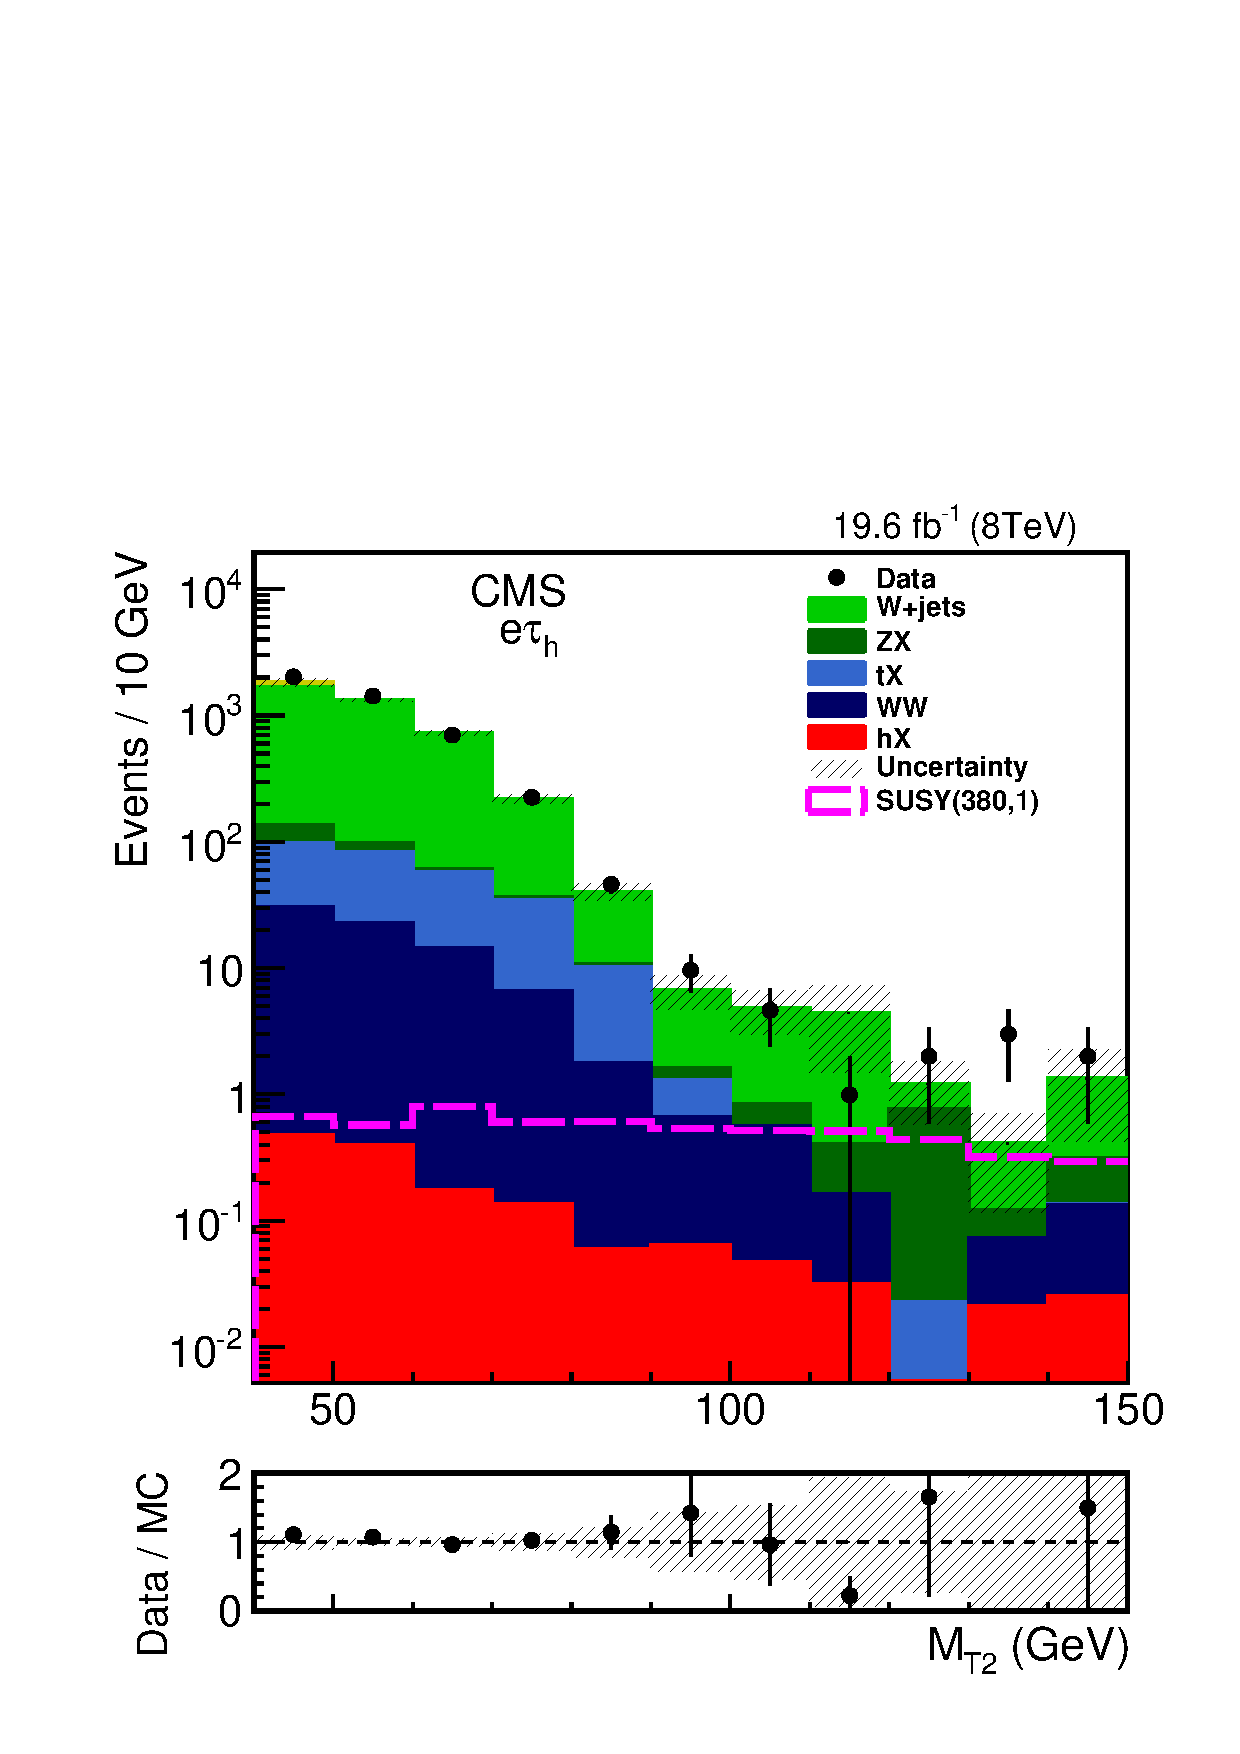
\includegraphics[angle=0,scale=0.375]{SelectionEleTau/MT2_eletau.pdf}
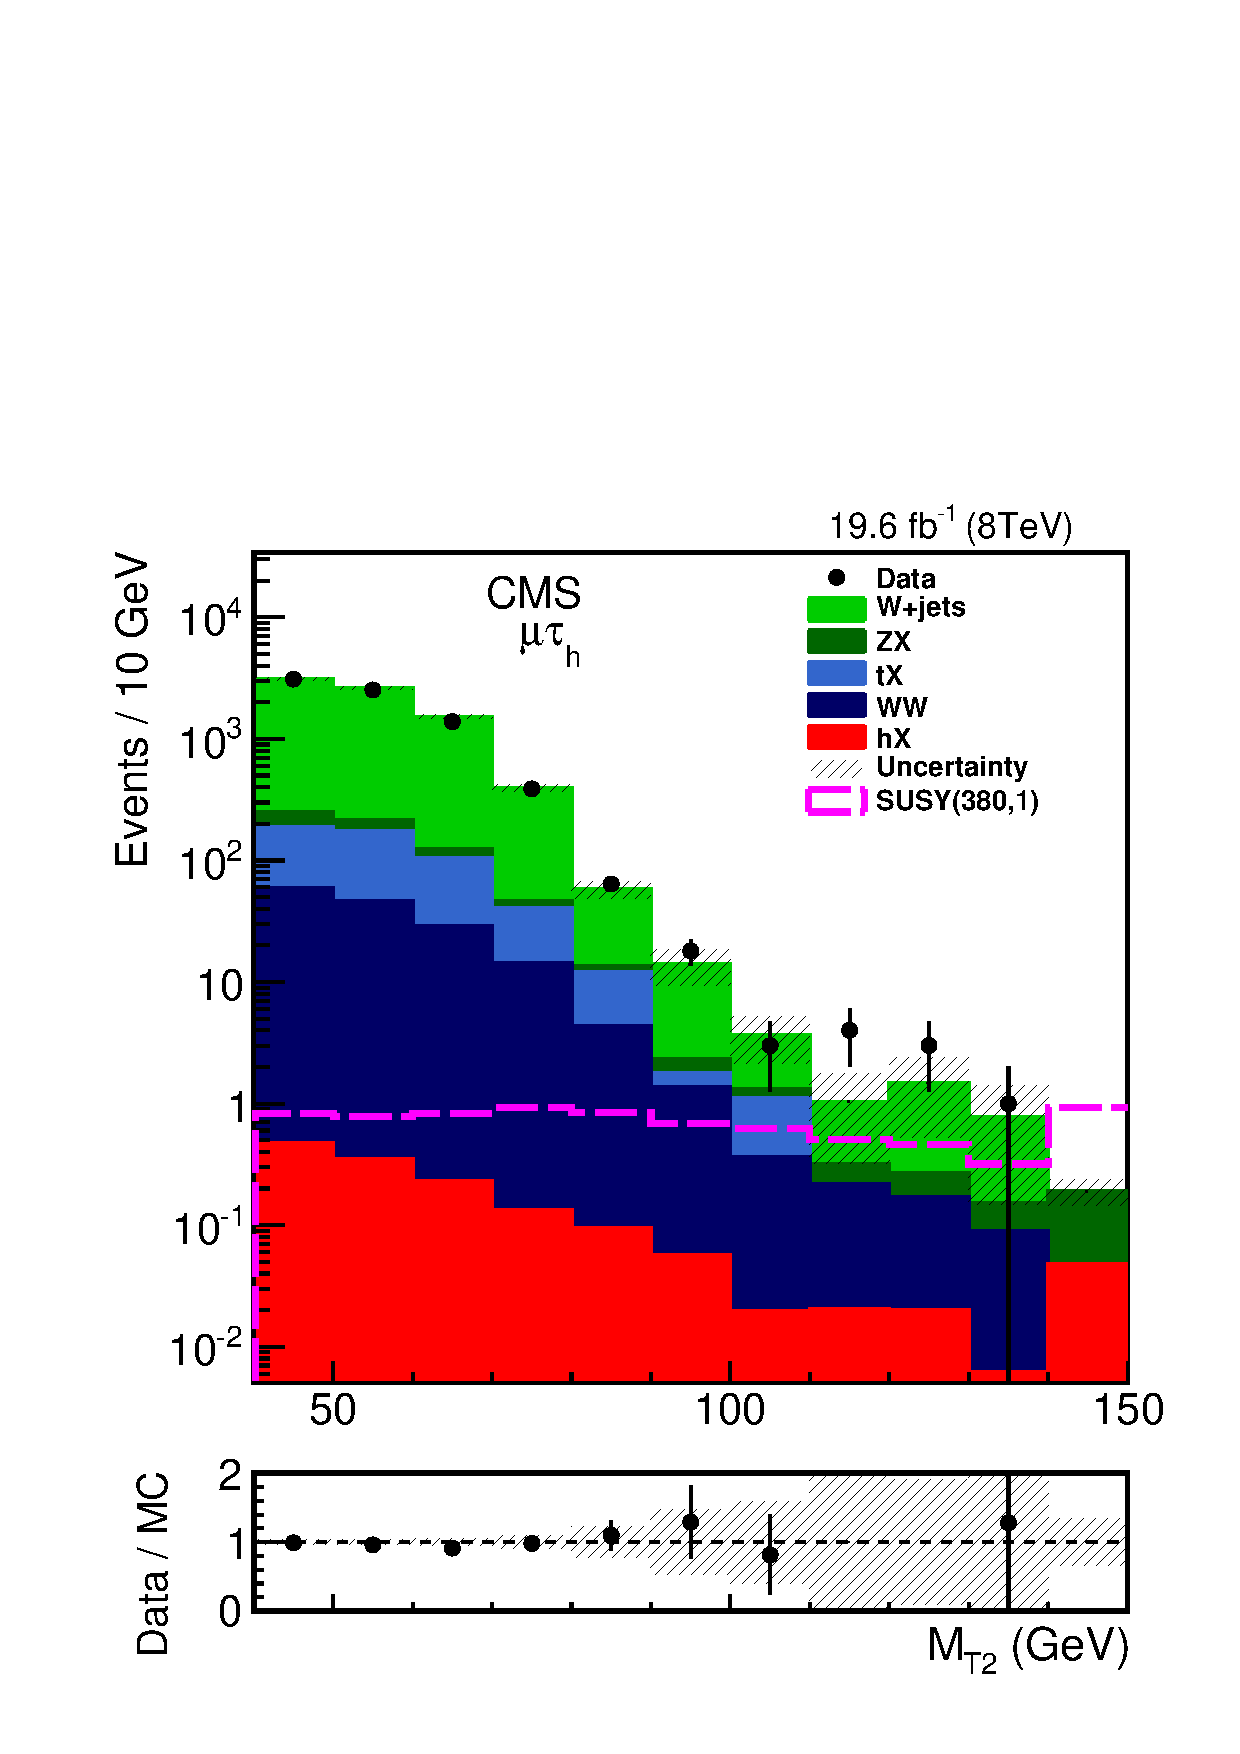
\includegraphics[angle=0,scale=0.375]{SelectionMuTau/MT2_mutau.pdf}
\caption{The \mttwo for events after the preselection, compared to SM expectation in (left) \eTau and (right) \muTau channels. The signal distribution is shown for $m_{\chione}=380\GeV,~m_{\PSGczDo}=1\GeV$. The last bins include the higher values of \mttwo also. Only the statistical uncertainties are shown.}
\label{fig:mt2leptontau}
\end{figure}






